\subsection{Ideal MHD Equations}

In DESC, we use the ideal MHD model for the plasma. So, the equations that we are solving are,
\begin{align}
    \textbf{Force Balance } &: \hspace{1cm} \J\times\B = \nabla p \label{eq_force}\\
    \textbf{Ampère's Law } &: \hspace{1cm} \nabla\times\B = \mu_0 \J \label{eq_amper}\\
    \textbf{Gauss's Law for Magnetism } &: \hspace{1cm} \nabla\cdot\B = 0 \label{eq_gauss}
\end{align}
We can write $\J$ from equation \ref{eq_amper}, and then equation \ref{eq_force} becomes,
\begin{equation}
    (\nabla\times\B)\times\B = \mu_0\nabla p   \label{force-error}
\end{equation}



% ===============================================================



\subsubsection{Magnetic Field}
Now, let's find the magnetic field in terms of flux coordinates $\rho, \theta$ and $\zeta$. Previously, we said that $\rho$ is a flux function but we didn't explain it. In DESC, we are assuming nested flux surfaces. So, we can use this property instead of radial distance. The flux surfaces can be labeled by the total enclosed toroidal flux. In DESC, we will use the following relation for $\rho$,
\begin{equation}
    \rho = \sqrt{\cfrac{\psi_T}{\psi_{T_{total}}}} \label{def_rho}
\end{equation}
We will use the contravariant form for the magnetic field,
\begin{equation}
    \B = B^\rho \e_\rho + B^\theta \e_\theta + B^\zeta \e_\zeta
\end{equation}
Due to the definition of flux surfaces, $\B\cdot\nabla\psi = 0$. Hence, $B^\rho = 0$ and 
\begin{equation}
    \B = B^\theta \e_\theta + B^\zeta \e_\zeta   \label{B_general}
\end{equation}
Substitute $\B$ in equation \ref{eq_gauss}, and use divergence in non-orthogonal coordinates \ref{cl-div},
\begin{equation}
    \cfrac{1}{\jac}\left(\cfrac{\partial(B^\theta\jac)}{\partial\theta} + \cfrac{\partial(B^\zeta\jac)}{\partial\zeta}\right) = 0
\end{equation}
This requires the term in parenthesis to be 0,
\begin{equation}
    \cfrac{\partial(B^\theta\jac)}{\partial\theta} = - \cfrac{\partial(B^\zeta\jac)}{\partial\zeta}  \label{condition}
\end{equation}
Let's try random functions for the solution,
\begin{align}
    B^\theta\jac &= A(\rho,\theta,\zeta) + a(\rho) \\
    B^\zeta\jac  &= C(\rho,\theta,\zeta) + c(\rho)
\end{align}
The functions that only depend on $\rho$ are added deliberately since these functions will cancel out for both partial derivatives of $\theta$ and $\zeta$, such that the equation \ref{condition} will be, 
\begin{equation}
    \cfrac{\partial A}{\partial\theta} = - \cfrac{\partial C}{\partial\zeta}
\end{equation}
Let's choose,
\begin{align}
    A(\rho,\theta,\zeta) = -f(\rho)\cfrac{\partial\lambda(\theta,\zeta)}{\partial\zeta} \hspace{.5cm}&\rightarrow\hspace{.5cm} \cfrac{\partial A}{\partial\theta} = -f(\rho)\cfrac{\partial^2\lambda}{\partial\theta\partial\zeta} \\
    C(\rho,\theta,\zeta) = f(\rho)\cfrac{\partial\lambda(\theta,\zeta)}{\partial\theta} \hspace{.5cm}&\rightarrow\hspace{.5cm} \cfrac{\partial C}{\partial\zeta} = f(\rho)\cfrac{\partial^2\lambda}{\partial\theta\partial\zeta}    
\end{align}
which satisfies our condition in the equation \ref{condition}. Then,
\begin{align}
    B^\theta\jac &= a(\rho) - f(\rho)\cfrac{\partial\lambda(\theta,\zeta)}{\partial\zeta} \\
    B^\zeta\jac  &= c(\rho) + f(\rho)\cfrac{\partial\lambda(\theta,\zeta)}{\partial\theta}
\end{align}
To find $a(\rho)$,  $c(\rho)$ and $f(\rho)$, we should look at the toroidal and poloidal fluxes which are given properties for equilibrium calculation. First, we will look at toroidal flux,
\begin{align}
    \psi_{T} &= \int \int B^\zeta \jac d\rho d\theta \\
    &= \int \int c(\rho')d\rho' d\theta + \int \left(\int_0^{2\pi}\dLt d\theta\right) f(\rho')d\rho' \\
    &= \int \int c(\rho')d\rho' d\theta + \int \mathlarger{(}\lambda(2\pi,\zeta) - \lambda(0,\zeta)\mathlarger{)}f(\rho')  d\rho' \\
    &= 2\pi \int_0^\rho c(\rho')d\rho'
\end{align}
In the third step, we could cancel the second integral because $\lambda$ is a periodic function. So, $\lambda(2\pi,\zeta) = \lambda(0,\zeta)$.
\begin{align}
    \psi_{T} &= 2\pi \int_0^\rho c(\rho')d\rho' \\
    c(\rho) &= \cfrac{1}{2\pi}\dFluxRho
\end{align}
I took the derivative of the first equation in terms of $\rho$. If we subsitute $c(\rho)$ in $B^\zeta$, we get,
\begin{equation}
    B^\zeta = \cfrac{1}{\jac}\left(\cfrac{1}{2\pi}\dFluxRho + f(\rho)\cfrac{\partial\lambda(\theta,\zeta)}{\partial\theta}\right)
\end{equation}
We can conduct similar steps for the poloidal flux,
\begin{align}
    \psi_P &= \int \int B^\theta \jac d\rho d\zeta \\
    &= \int \int a(\rho')d\rho' d\zeta - \int \left(\int_0^{2\pi}\dLzd\zeta\right) f(\rho')d\rho'  \\
    &= \int \int a(\rho')d\rho' d\zeta - \int \mathlarger{(} \lambda(\theta,2\pi) - \lambda(\theta,0)\mathlarger{)} f(\rho')d\rho'  \\
    &= 2\pi \int a(\rho')d\rho'
\end{align}
Again, I used the periodicity of $\lambda$,
\begin{align}
    \psi_P &= 2\pi \int_0^{\rho} a(\rho')d\rho' \\
    a(\rho) &= \cfrac{1}{2\pi}\cfrac{\partial \psi_P}{\partial\rho}
\end{align}
Remember that $\iota = \cfrac{\partial\psi_P/\partial\rho}{\partial\psi_T/\partial\rho}$. So,  $\partial\psi_P/\partial\rho = \iota$ $\partial\psi_T/\partial\rho$. Hence, $a(\rho)$ can be written as,
\begin{equation}
   a(\rho) = \cfrac{\iota}{2\pi}\cfrac{\partial \psi_T}{\partial\rho}
\end{equation}
If we subsitute $a(\rho)$ in $B^\theta$, we get,
\begin{equation}
    B^\theta = \cfrac{1}{\jac}\left(\cfrac{\iota}{2\pi}\dFluxRho - f(\rho)\cfrac{\partial\lambda(\theta,\zeta)}{\partial\zeta}\right)
\end{equation}
Finally, the magnetic field can be written as,
\begin{equation}
    \B = \cfrac{1}{\jac}\begin{bmatrix}
        \left(\cfrac{\iota}{2\pi}\dFluxRho - f(\rho)\cfrac{\partial\lambda(\theta,\zeta)}{\partial\zeta}\right)\e_\theta  +
        \left(\cfrac{1}{2\pi}\dFluxRho + f(\rho)\cfrac{\partial\lambda(\theta,\zeta)}{\partial\theta}\right) \e_\zeta
    \end{bmatrix}
\end{equation}
Since there is no constraint on $f(\rho)$, we can take it, for our convenience, as $f(\rho) = \cfrac{f^*(\rho)}{2\pi}\dFluxRho$ 
\begin{equation}
    \B = \cfrac{1}{\jac}\begin{bmatrix}
        \left(\cfrac{\iota}{2\pi}\dFluxRho - \cfrac{f^*(\rho)}{2\pi}\dFluxRho\cfrac{\partial\lambda(\theta,\zeta)}{\partial\zeta}\right)\e_\theta  +
        \left(\cfrac{1}{2\pi}\dFluxRho + \cfrac{f^*(\rho)}{2\pi}\dFluxRho\cfrac{\partial\lambda(\theta,\zeta)}{\partial\theta}\right) \e_\zeta
    \end{bmatrix}
\end{equation}
and we can include $f^*(\rho)$ inside $\lambda$. Then, we get,
\begin{equation}
    \B = \cfrac{1}{2\pi\jac}\dFluxRho\begin{bmatrix}
        \left(\iota - \cfrac{\partial\lambda(\rho,\theta,\zeta)}{\partial\zeta}\right)\e_\theta  +
        \left(1 + \cfrac{\partial\lambda(\rho,\theta,\zeta)}{\partial\theta}\right) \e_\zeta
    \end{bmatrix}  \label{mag_theta}  
\end{equation}
This last step may seem a bit arbitrary, but look what happens if we create a new coordinate system using $\vartheta = \theta + \lambda(\rho, \theta, \zeta)$. In DESC, this new coordinate is shown by $\vartheta$ or (vartheta), but due to its extreme similarity to $\theta$, I will use $\theta^*$ instead (s.t. $\theta^* = \theta + \lambda(\rho, \theta, \zeta)$). Let's write the basis vectors in the new coordinate frame,
\begin{align}
    \e_\theta|_{\rho,\zeta} = \cfrac{\partial \mathbf{R}}{\partial \theta} \hspace{1cm}&\rightarrow \hspace{1cm} \e_{\theta}|_{\rho,\zeta} = \cfrac{\partial \mathbf{R}}{\partial \theta^*}\cfrac{\partial \theta^*}{\partial \theta}  \\[.5cm]
    \e_{\theta}|_{\rho,\zeta} = \cfrac{\partial \mathbf{R}}{\partial \theta^*}\left(1+\dLt\right)\hspace{1cm}&\rightarrow \hspace{1cm} \boxed{\e_{\theta}|_{\rho,\zeta} = \left(1+\dLt\right)\e_{\theta^*}|_{\rho,\zeta}} \label{e_theta2star}
\end{align}
Here, the notation $\e_\theta|_{\rho,\zeta}$ is used to specify at which point the derivative is evaluated. We can follow similar steps for $\e_\zeta$,
\begin{align}
    \e_\zeta|_{\rho,\theta} = \cfrac{\partial \mathbf{R}}{\partial \zeta}|_{\rho,\theta} \hspace{1cm} &\rightarrow \hspace{1cm} 
    \e_\zeta|_{\rho,\theta} = \cfrac{\partial \mathbf{R}}{\partial \zeta}|_{\rho,\theta^*} + \cfrac{\partial \mathbf{R}}{\partial \theta^*}\cfrac{\partial \theta^*}{\partial \zeta} \\[.5cm]
    \e_{\zeta}|_{\rho,\theta} = \e_\zeta |_{\rho,\theta^*} + \cfrac{\partial (\theta + \lambda)}{\partial\zeta}\e_{\theta^*} |_{\rho,\zeta} 
    \hspace{1cm} &\rightarrow \hspace{1cm} \boxed{\e_\zeta |_{\rho,\theta} = \e_\zeta |_{\rho,\theta^*} + \dLz \e_{\theta^*} |_{\rho,\zeta}}  \label{e_zeta2star}
\end{align}
If we rewrite equation \ref{mag_theta} by specifying the previously hidden evaluation points,
\begin{equation}
    \B = \cfrac{1}{2\pi\jac}\dFluxRho\begin{bmatrix}
        \left(\iota - \dLz\right)\e_{\theta}|_{\rho,\zeta} + \left(1 + \dLt\right) \e_\zeta|_{\rho,\theta}
    \end{bmatrix}   \label{mag_theta_at} 
\end{equation}
Substitute \ref{e_theta2star} and \ref{e_zeta2star} in to this equation,
\begin{equation}
    \begin{split}
        \B &= \cfrac{1}{2\pi\jac}\dFluxRho\begin{bmatrix}
            \left(\iota - \dLz\right)\left(1+\dLt\right)\e_{\theta^*}|_{\rho,\zeta} + \left(1 + \dLt\right) \left(\e_\zeta |_{\rho,\theta^*} + \dLz \e_{\theta^*} |_{\rho,\zeta}\right)
        \end{bmatrix}   \\[0.3cm]
        &= \cfrac{1}{2\pi\jac}\left(1+\dLt\right)\dFluxRho\begin{bmatrix}
            \left(\iota - \dLz\right)\e_{\theta^*}|_{\rho,\zeta} + \e_\zeta |_{\rho,\theta^*} + \dLz \e_{\theta^*} |_{\rho,\zeta}
        \end{bmatrix}  \\[0.3cm]
        \B &= \cfrac{1}{2\pi\jac}\left(1+\dLt\right)\dFluxRho\left(            \iota  \e_{\theta^*}|_{\rho,\zeta} + \e_\zeta |_{\rho,\theta^*} \right)    \label{SFL-mag}
    \end{split}
\end{equation}
If we look at $B^{\theta^*}/B^{\zeta}$ ratio,
\begin{equation}
     \iota = \cfrac{B^{\theta^*}}{B^{\zeta}}
\end{equation}
As it turned out, if we use $\theta^*$ instead of $\theta$, the ratio of the magnetic field components gives rotational transform $\iota$. Therefore, in this new coordinate frame, the field lines appear straight and thus, it is called \textbf{straight field line coordinates} or SFL. If we draw the magnetic field in the $\theta$ direction versus the magnetic field in the $\zeta$ direction, we get a curve like the red solid line in the following Figure, 
\begin{figure}[H]
    \centering
    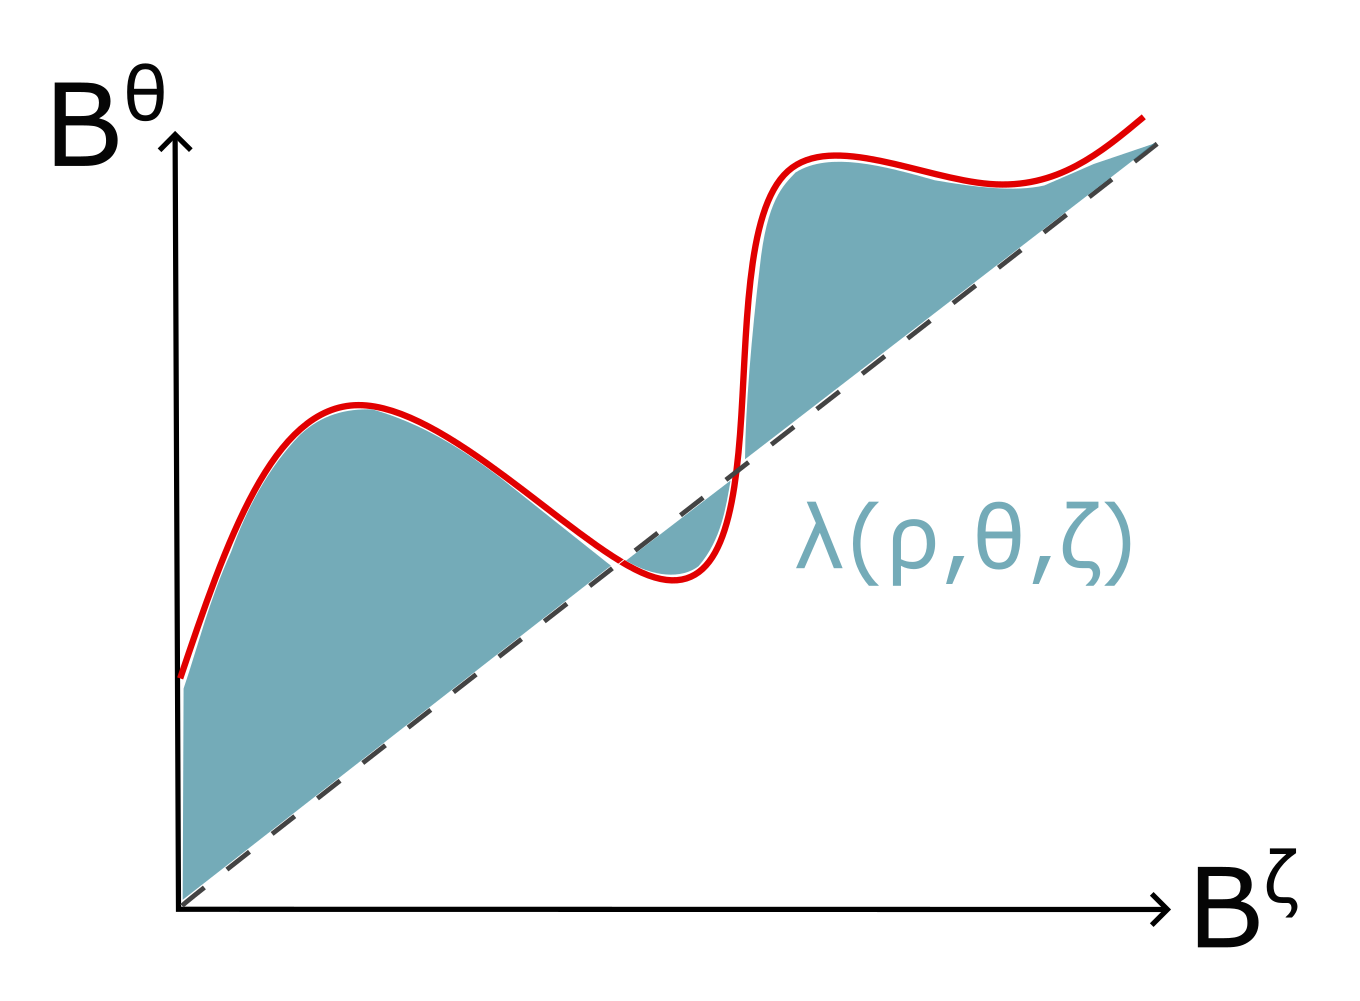
\includegraphics[width=8cm]{lambda-graph-2.png}
    \label{fig:enter-label}
\end{figure}
On the other hand, introducing $\lambda$ gives us the gray dashed line which has a known slope. {\color{red} THIS FIGURE MIGHT NOT MEAN WHAT I WANT IT TO - LOOK AGAIN}




% ===============================================================





\subsubsection{Electric Current Density}

We can write electric current density $\J$ in terms of $\B$ using equation \ref{eq_amper},
\begin{equation}
    \J = \frac{1}{\mu_0} \nabla \times \B
\end{equation}
We need to introduce the curl operator in curvilinear coordinates to calculate $\J$, which is,
\begin{equation}
    \nabla \times \B = \frac{1}{\jac} \sum_{k} \left( \frac{\partial B_j}{\partial u^i}  - \frac{\partial B_i}{\partial u^j}\right) \e_k
\end{equation}
where i, j and k are cyclic ([1,2,3], [2,3,1] or [3,2,1]), and here the indices stand for $\rho, \theta$, and $\zeta$. Plugging in the correct indices and expanding the equation, we can write the current density,
\begin{align}
    J^\rho &= \frac{\partial_\theta B_\zeta - \partial_\zeta B_\theta}{\mu_0 \jac} \\[.2cm]
    J^\theta &= \frac{\partial_\zeta B_\rho - \partial_\rho B_\zeta}{\mu_0 \jac} \\[.2cm]
    J^\zeta &= \frac{\partial_\rho B_\theta - \partial_\theta B_\rho}{\mu_0 \jac}
\end{align}
where,
\begin{align}
    B_\rho = \B \cdot \e_\rho = \Brho \\
    B_\theta = \B \cdot \e_\theta = \Btheta \\
    B_\zeta = \B \cdot \e_\zeta = \Bzeta
\end{align}
Notice that we have to find the covariant components of $\B$ to be able to find contravariant $\J$ components. 
\begin{align}
    B_\rho &= \Bvector \cdot \e_\rho \\
    B_\theta &= \Bvector \cdot \e_\theta \\
    B_\zeta &= \Bvector \cdot \e_\zeta
\end{align}
We will need some dot products like $\e_\rho \cdot \e_\theta$ and $\e_\rho \cdot \e_\zeta$,
\begin{align}
    \e_\rho \cdot \e_\theta &= \partial_\rho R \partial_\theta R + \partial_\rho Z \partial_\theta Z \\
    \e_\rho \cdot \e_\zeta &= \partial_\rho R \partial_\zeta R + \partial_\rho Z \partial_\zeta Z \\
    \e_\theta \cdot \e_\zeta &= \partial_\theta R \partial_\zeta R + \partial_\theta Z \partial_\zeta Z \\
    \e_\theta \cdot \e_\theta &= (\partial_\theta R)^2 + (\partial_\theta Z)^2 \\
    \e_\zeta \cdot \e_\zeta &= R^2 + (\partial_\zeta R)^2 + (\partial_\zeta Z)^2
\end{align}
Just for showing it one time, the full equations are,
\begin{equation}
    B_\rho = \cfrac{\dFluxRho}{2\pi\Jacobian}\begin{bmatrix}
        \left(\iota - \dLz\right) \left(\dRr \dRt + \dZr \dZt \right) + \left(1 + \dLt\right) \left(\dRr \dRz + \dZr \dZz \right)
    \end{bmatrix}
\end{equation}
\begin{equation}
    B_\theta = \cfrac{\dFluxRho}{2\pi\Jacobian}\begin{bmatrix}
        \left(\iota - \dLz\right) \left((\dRt)^2 + (\dZt)^2 \right) + \left(1 + \dLt\right) \left(\dRt \dRz + \dZt \dZz \right)
    \end{bmatrix}
\end{equation}
\begin{equation}
    B_\zeta = \cfrac{\dFluxRho}{2\pi\Jacobian}\begin{bmatrix}
        \left(\iota - \dLz\right) \left(\dRt \dRz + \dZt \dZz \right) + \left(1 + \dLt\right) \left(R^2 + (\dRz)^2 + (\dZz)^2 \right)
    \end{bmatrix}
\end{equation}

\subsubsection{$\J \times \B $ Force}
If we take the cross product of  $\J$  and $\B$ using equation \ref{cl-cross-contra} , we can write it as,
\begin{align}
    \J \times \B &= \jac \sum_k (J^i B^j - J^j B^i)\e^k \\
    &= \jac \begin{bmatrix}
        (J^\theta B^\zeta - J^\zeta B^\theta)\e^\rho  \hspace{.2cm}+\hspace{.2cm}
        (J^\zeta B^\rho - J^\rho B^\zeta)\e^\theta    \hspace{.2cm}+\hspace{.2cm}
        (J^\rho B^\theta - J^\theta B^\rho)\e^\zeta
    \end{bmatrix} \\
    &= \jac \begin{bmatrix}
        (J^\theta B^\zeta - J^\zeta B^\theta)\e^\rho  \hspace{.2cm}-\hspace{.2cm}
         J^\rho B^\zeta\e^\theta    \hspace{.2cm}+\hspace{.2cm}
         J^\rho B^\theta\e^\zeta
    \end{bmatrix} \\
    &= \jac (J^\theta B^\zeta - J^\zeta B^\theta)\e^\rho  \hspace{.2cm}-\hspace{.2cm}
       \jac J^\rho (B^\zeta\e^\theta - B^\theta\e^\zeta) \label{JcrossB}
\end{align}
I used $B^\rho$ = 0 (see \ref{appendix-1} for alternative). We can write the force error as,
\begin{equation}
    \mathbf{F} = \J \times \B - \nabla p
\end{equation}
Considering that pressure is a pure function of $\rho$, and using equation \ref{JcrossB},
\begin{align}
    \mathbf{F} = -\frac{\partial p}{\partial \rho} \nabla \rho + \jac (J^\theta B^\zeta - J^\zeta B^\theta)\e^\rho  -  \jac J^\rho (B^\zeta\e^\theta - B^\theta\e^\zeta)
\end{align}
Notice that $\nabla \rho = \e^\rho$,
\begin{align}
    \mathbf{F} = \left(-\frac{\partial p}{\partial \rho} + \jac (J^\theta B^\zeta - J^\zeta B^\theta) \right)\e^\rho  +  \jac J^\rho (B^\zeta\e^\theta - B^\theta\e^\zeta)
\end{align}
In DESC, we have the following notation for the force error,
\begin{equation}
    \mathbf{F} = F_\rho \e^\rho + F_\beta \mathbf{\beta_{DESC}}
\end{equation}
where,
\begin{align}
    F_\rho &=  \jac (J^\theta B^\zeta - J^\zeta B^\theta) -\frac{\partial p}{\partial \rho}\\[.3cm]
    F_\beta &=  \jac J^\rho \\[.3cm]
    \mathbf{\beta_{DESC}} &=  (B^\zeta\e^\theta - B^\theta\e^\zeta) 
\end{align}
Equivalently, we can substitute the formula for $\J$ and write,
\begin{align}
    F_\rho &=  B^\zeta \frac{\partial_\zeta B_\rho - \partial_\rho B_\zeta}{\mu_0} - B^\theta \frac{\partial_\rho B_\theta - \partial_\theta B_\rho}{\mu_0} -\frac{\partial p}{\partial \rho}\\[.3cm]
    F_\beta &=  \frac{\partial_\theta B_\zeta - \partial_\zeta B_\theta}{\mu_0} 
\end{align}
{\color{red} LIFE IS TOO SHORT TO EXPAND THESE EQUATIONS ! BUT IF I EVER FEEL THAT THIS MIGHT HELP, I CAN EXPAND THEM SOME DAY}
